\documentclass[twoside,11pt]{homework}
\usepackage{graphicx}
\usepackage{booktabs}
\usepackage{lipsum}
\usepackage{indentfirst}

\coursename{COMS 4771 Machine Learning (Spring 2015)} % DON'T CHANGE THIS

\studname{Jingwei Yang}    % YOUR NAME GOES HERE
\studmail{jy2653@columbia.edu}% YOUR UNI GOES HERE
\hwNo{1}                   % THE HOMEWORK NUMBER GOES HERE
\collab{mw2972,yd2300}   % THE UNI'S OF STUDENTS YOU DISCUSSED WITH
\begin{document}
\maketitle

\section*{Problem 1}
\indent
1.   Training error:  14.00\%,   test error: 15.90\%.\\

\indent
2.   When I apply hw1\_train1a and hw1\_test1a over the OCR training data, I keep on receiving the warning message of "Matrix is singular to working precision".  The reason for this warning is that: the determinant of covariance matrix is 0 for each estimated covariance matrix, thus the matrix is not invertible. In Matlab, the forced inversion over the not invertible matrix could lead to a matrix filled with Infinity value, thus I received the warning of "Matrix is singular to working precision" when I use the inverted matrix to make predication.\\

\indent
3.  In this part, I replace the estimated covariance matrix in part2 with identity matrix in the classifier. The result: training error: 19.20\%, test error: 17.97\%. Because the identity matrix is invertible, I no longer received the warning in part2. But,  I get the error rate of extraordinarily  high, the disappointing error rate is caused by I directly take exponential over the part:
$\exp(-\frac{1}{2}(x - \hat{u}_y)^\top \sum ^ {-1}(x - \hat{u}_y))$.  Therefore I take the logarithm of the classifier, and get the right classification. 

% YOUR SOLUTION GOES HERE
\section*{Problem 2}
\begin{center}
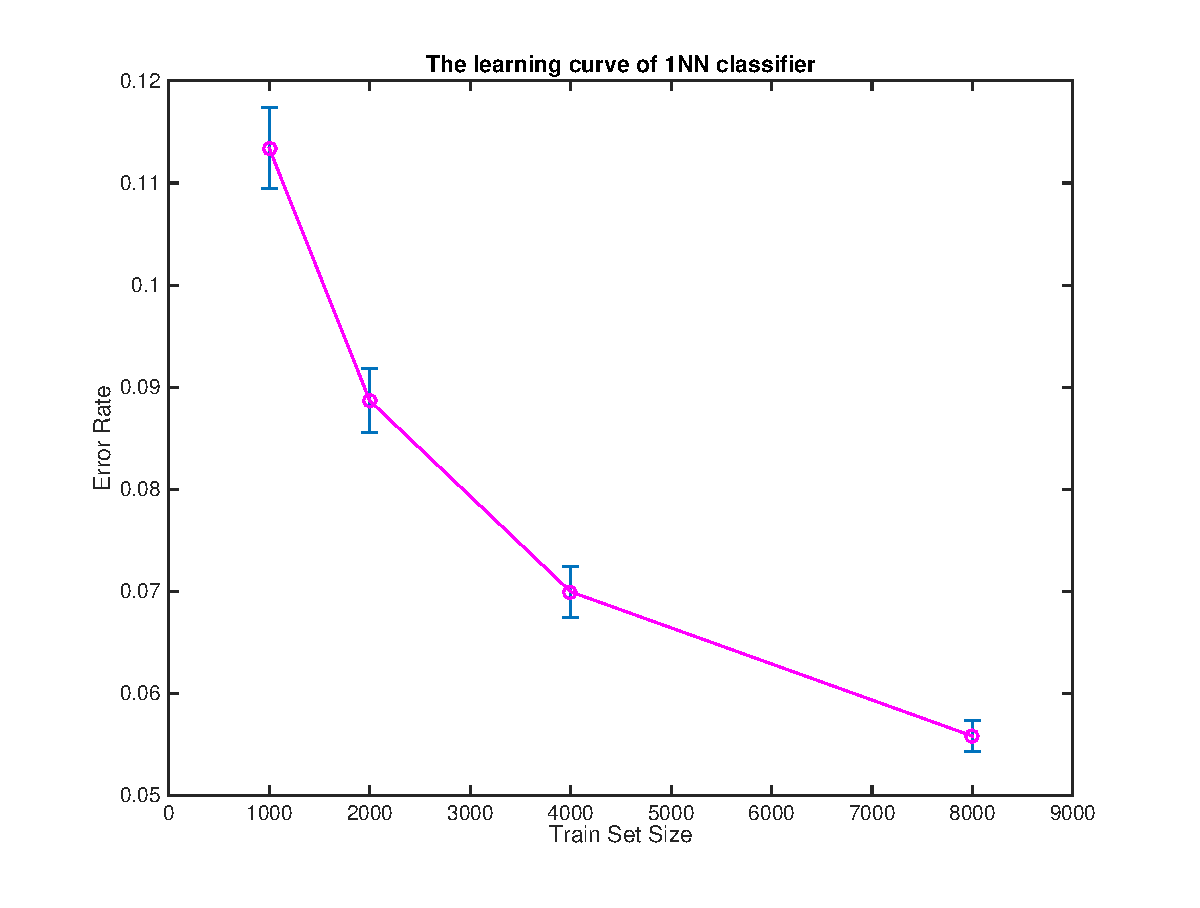
\includegraphics[width=150mm, height = 100mm]{learningcurve.eps}

\begin{table}[h]
\caption {The error rate table} \label{tab:title}
\centering
\begin{tabular}{@{}lrrrr@{}}
\toprule
train set  size                        & 1000    & 2000    & 4000    & 8000    \\ \midrule
error  rate                            & 0.11341 & 0.08869 & 0.06996 & 0.05582 \\ \midrule
standard deviation              & 0.00397 & 0.00316 & 0.00248 & 0.00148
\end{tabular}

\end{table}
\end{center}




% YOUR SOLUTION GOES HERE
\section*{Problem 3}

\indent
According to the problem, we have following cost function $cost(f(X), Y)$.
\[
cost(f(X), Y) =
\begin{cases} 
c & f(X) = 1, Y = 0 \\ 
1 & f(X) = 0, Y = 1 \\
0 & f(X) = Y
\end{cases}
\] \\
Suppose $(X, Y) \sim P$, For any classifier $f: X \rightarrow Y$, its expected classification cost is:
\[
E[cost(f(X) \neq Y)]  = E[E[cost(f(X) \neq Y)|X] ]
\] 
For each $x \in X$,
\[
E[E[cost(f(X) \neq Y)|X]]= Pr[Y=0|X=x]*cost(f(x)\neq y)+ Pr[Y=1|X=x]*cost(f(x)\neq y)
\] 

To minimize the cost,
\[
f(x) = \underset {y \in {0, 1}}{argmin} (Pr[Y=0|X=x]*c ,  Pr[Y=1|X=x]*1)
\] 
By Bayes' rule:
\[
Pr[Y=y|X=x] = \frac{Pr[Y=y]\cdot Pr[X=x|Y=y]} {Pr[X=x]}
\] 
We have:
\[
f(x) = \underset {y \in {0, 1}}{argmin} (Pr[Y=0]\cdot Pr[X=x|Y=0]*c ,  Pr[Y=1]\cdot Pr[X=x|Y=1])
\] 
Since we have $Pr(Y=0) = 2/3$ and $Pr(Y=1) = 1/3$, and class conditional densities are $N(0,1)$ for class 0, and $N(1, 1/4)$ for class 1. We have the classifier:
\[
f(x) =
\begin{cases} 
1 & c\cdot exp(-\frac{x^2}{2}) < exp(-2(x-1)^2) \\
0 & other
\end{cases}
\] \\
\end{document} 